\title{%
  A High-Level Overview of Cryptography
}
\author{%
  Daniel Bosk
}
\institute[KTH/MIUN]{%
  School of Computer Science and Communication,\\
  KTH Royal Institute of Technology, Stockholm
  \and
  Department of Information and Communication Systems,\\
  Mid Sweden University, Sundsvall
}
\date{\today}

\maketitle

\mode*

\begin{abstract}
  Cryptography has a central role in security.
To fully understand how many security mechanisms can be implemented we need 
cryptography.
For this reason, we also need higher-level knowledge about what can be achieved 
with cryptography to not limit our thoughts about possible solutions.
This learning session is intended to give a high-level overview of 
cryptography: \ac{SKE}, \ac{PKE}, digital signatures, \ac{ZKP} and \ac{MPC}.
In particular, the \acp{ILO} are that you should be able to
\begin{itemize}
  \item \emph{understand} what properties can be achieved with cryptography.
  \item \emph{analyse} a situation and \emph{suggest} what cryptographic 
    properties are desirable.
\end{itemize}

We will treat
Chapter 5 in Anderson's \citetitle{Anderson2008sea}~\cite{Anderson2008sea} and
Chapter 14 in Gollmann's \citetitle{Gollmann2011cs}~\cite{Gollmann2011cs}.
To practice your understanding of these mechanisms it is recommended to do 
exercises 14.2, 14.3 and 14.7 in~\cite{Gollmann2011cs}.
We will also cover some topics from 
\citetitle{Katz-Lindell}~\cite{Katz-Lindell} and 
\citetitle{GoldreichFOC-1}~\cite{GoldreichFOC-1}.

\end{abstract}


% Since this a solution template for a generic talk, very little can
% be said about how it should be structured. However, the talk length
% of between 15min and 45min and the theme suggest that you stick to
% the following rules:  

% - Exactly two or three sections (other than the summary).
% - At *most* three subsections per section.
% - Talk about 30s to 2min per frame. So there should be between about
%   15 and 30 frames, all told.


\section{Introduction}

\subsection{History}

\begin{frame}
  \begin{itemize}
    \item The word has its origin in greek~\footfullcite{OED2013cg}:
      \begin{description}
        \item[\ibygr{krupto's}] (\emph{kryptos}) meaning 
          hidden~\footfullcite{OED2013c}.
        \item[\ibygr{gra'fos}] (\emph{graphos}) meaning 
          writing~\footfullcite{OED2013g}.
      \end{description}

      \pause{}

    \item The area has been around for ages.

      \pause{}

    \item We should not confuse it with \emph{steganography}.
    \item Steganography concerns hiding a message's \emph{existence}.
    \item Cryptography concerns hiding a message's \emph{contents}.

  \end{itemize}
\end{frame}

\begin{frame}
  \begin{itemize}
    \item Then it was an art, now it's a science.

      \pause{}

    \item People used \enquote{clever} constructions.
    \item These were thought to be secure: \enquote{How can anyone figure this 
        out?}

      \pause{}

    \item Well, it turns out that there are always a lot of people with a lot 
      of time and motivation \dots
  \end{itemize}
\end{frame}

\subsection{Kerckhoff's Principle}

\begin{frame}
  \begin{block}{A quote\footfullcite{KerckhoffsPrinciple}}
    \begin{displayquote}\relax
      [A cryptosystem] should not require secrecy, and it should not be 
      a problem
      if it falls into the enemy hands;
    \end{displayquote}
  \end{block}

  \pause{}

  \begin{block}{Kerckhoff's Principle}
    \begin{itemize}
      \item No security-by-obscurity
      \item The key should be the only secret
    \end{itemize}
  \end{block}
\end{frame}

\begin{frame}
  \begin{itemize}
    \item This doesn't mean we have to tell the adversary what we're using.
    \item But we shouldn't loose any security if we do.
  \end{itemize}
\end{frame}


\section{Symmetric Cryptography}

\subsection{Ciphers}

\begin{frame}
  \begin{block}{The idea}
    \begin{itemize}
      \item Alice and Bob share a (small) common secret.

        \pause{}

      \item Alice takes a message, combines it with the secret, sends it to 
        Bob.

        \pause{}

      \item If Eve captures the whatever Alice sent, she shouldn't learn 
        anything about the message.

        \pause{}

      \item Bob combines what he received with the secret and gets the message.
    \end{itemize}
  \end{block}
\end{frame}

\begin{frame}
  \begin{block}{Block-cipher encryption}
    \begin{description}
      \item[Input] A fixed-sized \emph{key} \(\Key{}\), a fixed-sized block of 
        \emph{plaintext} \(p\).
      \item[Output] A fixed-sized block of \emph{ciphertext} \(c\).
      \item[Notation] \(\Enc[\Key{}]{p} = c\)
    \end{description}
  \end{block}

  \pause{}

  \begin{block}{Block-cipher decryption}
    \begin{description}
      \item[Input] A fixed-sized \emph{key} \(\Key{}\), a fixed-sized block of 
        \emph{ciphertext} \(c\).
      \item[Output] A fixed-sized block of \emph{plaintext} \(p\).
      \item[Notation] \(\Dec[\Key{}]{c} = p\)
    \end{description}
  \end{block}
\end{frame}

\begin{frame}
  \begin{definition}[Crypto 
    system\footfullcite{Stinson2006cta}]\label{CryptoSystem}
    \begin{itemize}
        \item A \emph{crypto system} is a tuple \((\M, \C, \K, \E, \D)\), 
          where:
          \begin{itemize}
            \item \(\M\) is a finite set of \emph{plaintexts} or messages,
            \item \(\C\) is a finite set of \emph{ciphertexts},
            \item \(\K\) is the \emph{keyspace}, a finite set of keys.
            \item \(\E\) and \(\D\) are the sets of encryption and decryption
              rules, respectively.
          \end{itemize}

          \pause{}

        \item For every \(k\in \K\) there is a \(\Enc[k]{}\in \E\) and 
          \(\Dec[k]{}\in \D\) such that
          \begin{itemize}
            \item \(\Enc[k]{}\colon \M\to \C\) and \(\Dec[k]{}\colon \C\to 
                \M\) are functions and
            \item \(\Dec[k]{\Enc[k]{m}} = m\) for all plaintexts \(m\in 
                \M\).
          \end{itemize}
      \end{itemize}
  \end{definition}
\end{frame}

\begin{frame}
  \begin{definition}[Shift Cipher]\label{ShiftCipher}
    \begin{itemize}
      \item Let \(\M = \C = \K = \Z_{29}\)
      \item For each \(k\in \K\) we define
        \begin{align}
          \nonumber
          \Enc[k]{m} &= (m + k) \bmod 29, m\in \M, \text{\ och } \\
          \nonumber
          \Dec[k]{c} &= (c - k) \bmod 29, c\in \C.
        \end{align}
    \end{itemize}
  \end{definition}

  \pause{}

  \begin{example}
    \begin{itemize}
      \item \(\Enc[3]{7} = 7+3 \bmod 29 = 10\)\hfill h\(\to\)J
      \item \(\Enc[3]{4} = 4+3 \bmod 29 = 7\)\hfill e\(\to\)G
      \item \(\Enc[3]{9} = 9+3 \bmod 29 = 12\)\hfill j\(\to\)L
    \end{itemize}
  \end{example}
\end{frame}

\begin{frame}
  \begin{exercise}
    \begin{itemize}
      \item What do we have to do to set this up between two parties, say Alice 
        and Bob?
      \item What problems do we have to solve?
    \end{itemize}
  \end{exercise}
\end{frame}

\subsection{Security}

\begin{frame}
  \begin{definition}[Perfect secrecy~\footfullcite{ShannonSecrecy}]
    \begin{itemize}
      \item Cryptosystem \((\M, \C, \K, \E, \D)\).
      \item Stochastic variables \(M, C\).
      \item \emph{Perfect secrecy} if and only if \[\Pr(M = m\mid C = c) 
          = \Pr(M = m)\] for all \(m\in \M\) and \(c\in \C\).
    \end{itemize}
  \end{definition}

  \pause{}

  \begin{block}{Note}
    Equivalent to \(H(M\mid C) = H(M)\), i.e.\ ciphertext does not reveal 
    anything about plaintext.
  \end{block}
\end{frame}

\begin{frame}
  \begin{theorem}[Shannon's theorem]
    \begin{itemize}
      \item Assume cryptosystem \((\M, \C, \K, \E, \D)\) such that \(|\K| 
          = |\C| = |\M|\).

        \pause{}

      \item This provides perfect secrecy if and only if
        \begin{enumerate}
          \item every key \(k\in \K\) is used with equal probability 
            \(1/|\K|\),
          \item for every plaintext \(m\in \M\) and \(c\in \C\) there is 
            a unique key such that \(\Enc[k]{m} = c\).
        \end{enumerate}
    \end{itemize}
  \end{theorem}
\end{frame}

\begin{frame}
  \begin{example}[One-time Pad]
    \begin{itemize}
      \item Let \(n\) be a positive integer.
      \item Let \(\M = \C = \K = (\Z_2)^n\).

        \pause{}

      \item For each key \(k = (k_1, \ldots, k_n)\in \K\), plaintexts \(m 
          = (m_1, \ldots, m_n)\in \M\) and ciphertexts \(c = (c_1, \ldots, 
          c_n)\in \C\) we define
        \[\Enc[k]{m} = (m_1 + k_1, \ldots, m_n + k_n)\]

        \pause{}

      \item We also define \(\DecOp = \EncOp\).

        \pause{}

      \item \(k\in \K\) must be chosen uniformly randomly for each encryption.
    \end{itemize}
  \end{example}
\end{frame}

\begin{frame}
  \begin{definition}[\Acl{PRP}, \acs{PRP}\footfullcite{KatzLindell-v1}]
    \begin{itemize}
      \item Let \(F\colon \{0,1\}^s\times \{0, 1\}^n\to \{0,1\}^n\).

        \pause{}

      \item \(F\) is \iac{PRP} if
        \begin{enumerate}
          \item for any \(k\in \{0, 1\}^s\), \(F\) is a bijection;

            \pause{}

          \item for any \(k\in \{0, 1\}^s\), we can \enquote{efficiently} 
            evaluate \(F_k(x)\);

            \pause{}

          \item for all \enquote{efficient} distinguishers \(D\),
            \[\left|\Pr[D^{F_k}(1^n) = 1] - \Pr[D^{f_n}(1^n) = 1]\right| 
              < \epsilon(s)\] if we choose \(k\in \{0,1\}^s\) and the random 
            permutation \(f_n\) uniformly at random.
        \end{enumerate}
    \end{itemize}
  \end{definition}
\end{frame}

\subsection{Hash Functions}

\begin{frame}
  \begin{block}{The idea}
    \begin{itemize}
      \item We want a function which we can efficiently compute.

        \pause{}

      \item However, it shouldn't be possible to find its inverse.
    \end{itemize}
  \end{block}

  \pause{}

  \begin{example}
    \begin{description}
      \item[Easy] \(f(x) = y\)
      \item[Hard] \(f^{-1}(y) = x\)
    \end{description}
  \end{example}
\end{frame}

\begin{frame}
  \begin{figure}
    \subfloat[\(h\colon X\to Y\)]{%
      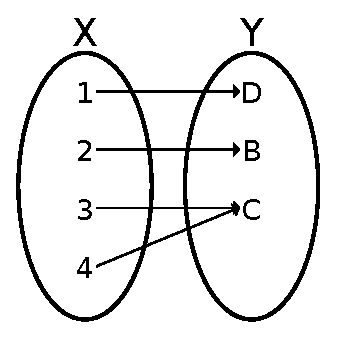
\includegraphics[height=2cm]{surjection.eps}%
    }
    \hspace{0.1\textwidth}
    \subfloat[\(h^\prime\colon X\to Y\)]{%
      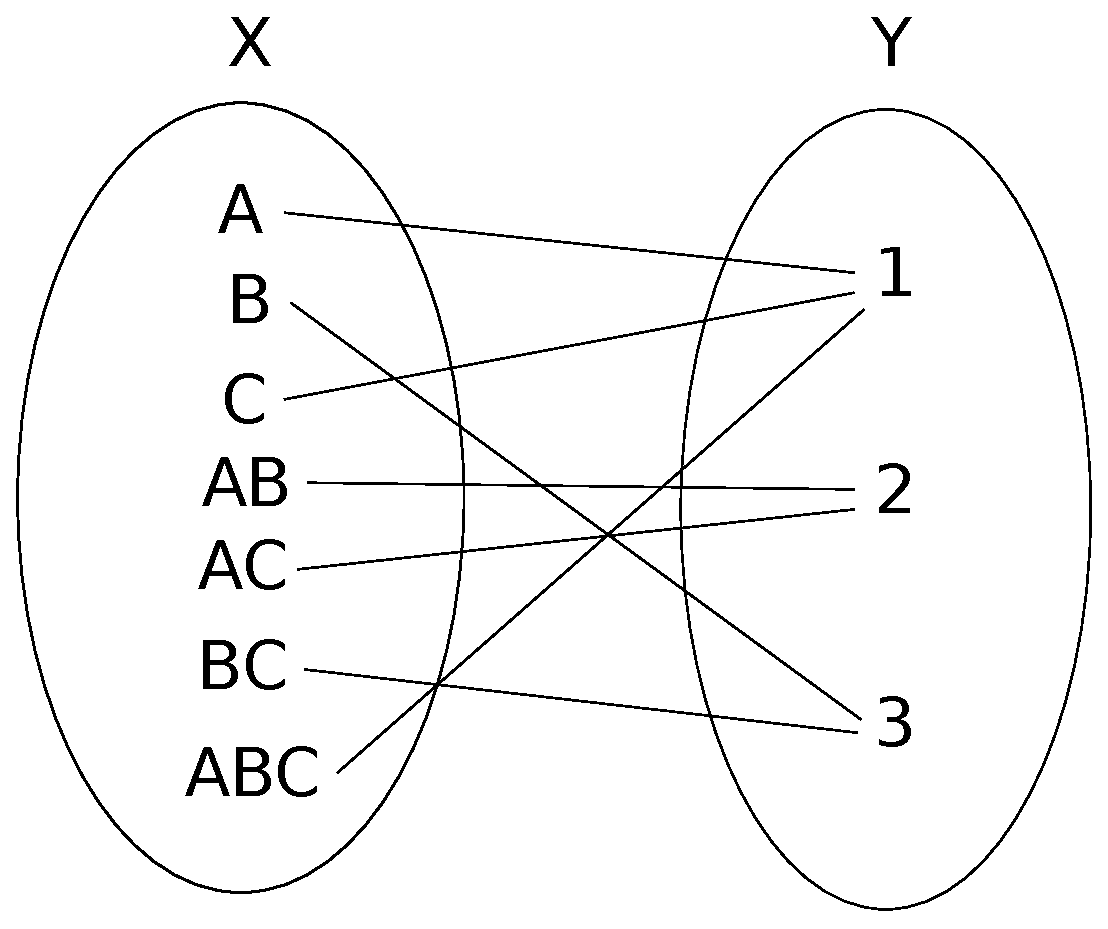
\includegraphics[height=2cm]{hashfunc.eps}%
    }
    \caption{%
      Two non-injective, surjective functions \(h\) and \(h^\prime\).
    }
  \end{figure}

  \begin{exercise}
    Could either of these two functions be one-way functions?
  \end{exercise}
\end{frame}

\begin{frame}
  \begin{definition}[One-way function\footfullcite{GoldreichFOC-1}]
    \begin{itemize}
      \item Let \(h\colon \{0,1\}^*\to \{0,1\}^*\).
      \item \(h\) is \emph{one-way} if
        \begin{enumerate}
          \item there exists an efficient algorithm \(A\) such that \(A(x) 
              = h(x)\);
          \item for every efficient algorithm \(A^\prime\), every positive 
            polynomial \(p(\cdot)\) and all sufficiently large \(n\)'s
            \[\Prob{A^\prime(h(x), 1^n) \in h^{-1}(h(x))} < \frac{1}{p(n)}\]
        \end{enumerate}
    \end{itemize}
  \end{definition}
\end{frame}

\begin{frame}
  \begin{example}[Implementations you might've heard of]
    \begin{itemize}
      \item MD5
      \item SHA1
      \item SHA256 (SHA-2)
      \item SHA-3
    \end{itemize}
  \end{example}
  \begin{example}[Applications]
    \begin{itemize}
      \item Verifying file content integrity
      \item Digital signatures
      \item Protect passwords
    \end{itemize}
  \end{example}
\end{frame}

\subsection{\Aclp{MAC}}

\begin{frame}
  \begin{example}
    \begin{itemize}
      \item Let \(\Enc[k]{\cdot} = \Dec[k]{\cdot} = \cdot\oplus k\bmod 2\).
        
        \pause{}

      \item Alice and Bob share \(k\).
      \item Alice sends \(\Enc[k]{m} = c\) to Bob.

        \pause{}

      \item Eve intercepts \(c\), she cannot get to \(m\).

        \pause{}

      \item Eve computes \(c^\prime = c\oplus m_E\) and passes \(c^\prime\) to 
        Bob.

        \pause{}

      \item Bob computes \(\Dec[k]{c^\prime} = \Dec[k]{c\oplus m_E} = m\oplus 
          k\oplus m_E\oplus k = m\oplus m_E\).
    \end{itemize}
  \end{example}

  \pause{}
  
  \begin{exercise}
    How can we solve this?
    Bob needs to know that Eve modified the message!
  \end{exercise}
\end{frame}

\begin{frame}
  \begin{block}{The idea: \acp{MAC}}
    \acuse{MA}
    \begin{itemize}
      \item Alice and Bob need something that Eve doesn't know how to modify.

        \pause{}

      \item If that something is tied to the message, then a modified message 
        would be detectable.
    \end{itemize}
  \end{block}

  \pause{}

  \begin{exercise}
    Any ideas on how we can construct such a thing?
  \end{exercise}
\end{frame}

\begin{frame}
  \begin{example}
    \begin{itemize}
      \item Let \(h\) be a one-way function.
        
        \pause{}
        
      \item If we use \(h(c) = t\), then Eve can also compute the hash 
        function: \(h(c^\prime) = t^\prime\).

        \pause{}

      \item A secret hash function would violate Kerckhoff's principle, so 
        that's not an option.

        \pause{}

      \item If we instead use the message, rather than the ciphertext.
        
      \item Then \(h(m) = t\) and
        \begin{itemize}
          \item \(\Dec[k]{c^\prime} = m^\prime = m\oplus m_E, h(m^\prime)\neq 
              t\).
          \item \(\Dec[k]{c} = m, h(m) = t\).
        \end{itemize}

        \pause{}
        
      \item Eve cannot compute the hash function, she doesn't have \(m\)!
        \pause{}
        \begin{itemize}
          \item Bob: But neither do I\@!
        \end{itemize}
    \end{itemize}
  \end{example}

  \pause{}

  \begin{exercise}
    Any better ideas?
  \end{exercise}
\end{frame}

\begin{frame}
  \begin{solution}
    \begin{itemize}
      \item Let \(s\) be a secret shared between Alice and Bob.

        \pause{}

      \item \(h(c\concat s) = t\), Eve doesn't know \(s\).
      \item Bob can immediately check \(h(c^\prime\concat s)\neq t\).
    \end{itemize}
  \end{solution}

  \pause{}

  \begin{alertblock}{Note}
    \begin{itemize}
      \item It requires even a bit more than this!
      \item But the idea is correct.
    \end{itemize}
  \end{alertblock}
\end{frame}

\begin{frame}
  \begin{solution}[\Acl{HMAC}, \acs{HMAC}\footfullcite{HMAC}]
    \begin{itemize}
      \item Let \(h\) be a one-way function.
      \item Let \(c\) be the ciphertext, \(s\) our \ac{MA} secret.

        \pause{}

      \item Then tag \(t = \HMAC[s]{c}\), where \[
          \HMAC[s]{c} = h\left[
            (s\oplus p_o)\concat h\left[ (s\oplus p_i)\concat c \right]
          \right],
        \] and \(p_i, p_o\) are inner and outer pads, respectively.
    \end{itemize}
  \end{solution}

  \pause{}

  \begin{alertblock}{Note}
    This is proven secure!
  \end{alertblock}
\end{frame}


\section{Public-Key Cryptography}

\subsection{Key-Exchange Schemes}

\begin{frame}
  \begin{block}{The idea}
    \begin{itemize}
      \item It's difficult to have to exchange keys in advance.

        \pause{}

      \item What if we could securely exchange keys at a distance?
      \item If we could do it just before we use them?
    \end{itemize}
  \end{block}

  \pause{}

  \begin{exercise}
    \begin{itemize}
      \item Say Alice and Bob want to communicate.
      \item Eve wants to eavesdrop as usual.
      \item What are the requirements of such a system?
    \end{itemize}
  \end{exercise}
\end{frame}

\begin{frame}
  \begin{solution}[Requirements]
    \begin{itemize}
      \item We need a problem that is easy for Alice and Bob.
      \item It should be hard for Eve.
    \end{itemize}
  \end{solution}
\end{frame}

\begin{frame}
  \begin{definition}[\Acl{DLP}, \acs{DLP}]
    \begin{itemize}
      \item Let \(\Z_p^*\) be the multiplicative group of residues modulo 
        \(p\in \N\), where \(p\) is a prime.

        \pause{}

        \begin{description}
          \item[Given] \(g, g^x\in \Z_p^*\)
          \item[Find] \(x\).
        \end{description}

      \item I.e.\ compute \(\log_{g\in \Z_p}(g^x)\).
    \end{itemize}
  \end{definition}
\end{frame}

\begin{frame}
  \begin{definition}[\Acl{DHP}, \acs{DHP}\footfullcite{DiffieHellman}]
    \begin{description}
      \item[Given] \(g, g^x, g^y\in \Z_p^*\)
      \item[Find] \(g^{xy}\)
    \end{description}
  \end{definition}

  \pause{}
  
  \begin{definition}[\Acl{DDH} Problem, \acs{DDH}]
    \begin{description}
      \item[Given] \(g, g^x, g^y, g^z\in \Z_p^*\)
      \item[Decide] \(z \stackrel{?}{=} xy\)
    \end{description}
  \end{definition}
\end{frame}

\begin{frame}
  \begin{itemize}
    \item If we can solve \ac{DLP}, then we can solve \ac{DHP} and \ac{DDH} 
      too.

      \pause{}

    \item Maybe \ac{DHP} and \ac{DDH} can be solved without \ac{DLP}.
    \item We don't know yet.

      \pause{}

    \item We usually assume \ac{DLP}, \ac{DHP} and \ac{DDH} are hard.
  \end{itemize}
\end{frame}

\begin{frame}
  \begin{exercise}
    \begin{itemize}
      \item \citeauthor{DiffieHellman}\footfullcite{DiffieHellman} used 
        \ac{DHP} to create a key-exchange protocol.

        \pause{}

      \item Take some time to figure out how we can use these problems to 
        achieve what we want.
    \end{itemize}
  \end{exercise}

  \begin{block}{Reminder}
    \begin{itemize}
      \item Alice and Bob want to exchange a secret key.
      \item Then they can use the key to encrypt their communications.
    \end{itemize}
  \end{block}
\end{frame}

\begin{frame}
  \begin{definition}[Diffie-Hellman key-exchange]
    \begin{itemize}
      \item Let \(g\in \Z_p^*\).

        \pause{}

      \color{green!50!red}
      \item Alice generates random \(0 < x < |\Z_p^*|\).
      \item She send \(g^x\) to Bob.

        \pause{}

      \color{blue}
      \item Bob generates random \(0 < y < |\Z_p^*|\).
      \item He sends \(g^y\) to Alice.

        \pause{}

      \color{green!50!red}
      \item Alice has \(x\) and \(g^y\).
      \color{blue}
      \item Bob has \(g^x\) and \(y\).
      \color{black}
      \item They both compute \(g^{xy} = {\color{green!50!red} (g^y)^x} 
          = {\color{blue} (g^x)^y}\).

        \pause{}

      \color{red}
      \item Eve has \(g^x, g^y\).
      \item By \ac{DHP} she cannot compute \(g^{xy}\).
    \end{itemize}
  \end{definition}
\end{frame}

\subsection{Encryption and Decryption}

\begin{frame}
  \begin{block}{The idea}
    \begin{itemize}
      \item Fine, we can use \(g^{xy}\) as a key in a cipher.
        \begin{itemize}
          \item \(\Enc[g^{xy}]{m}\), where \(\EncOp\) is a symmetric cipher.
        \end{itemize}
      \item But shouldn't we be able to include a message directly?
    \end{itemize}
  \end{block}
\end{frame}

\begin{frame}
  \begin{definition}[ElGamal Encryption Scheme\footfullcite{ElGamal}]
    Set-up:
    \begin{itemize}
      \item Let \(g\in \Z_p^*\), randomly choose \(0 < x < |\Z_p^*|\).
      \item Alice publishes \(\Z_p^*, g, g^x\) to everyone.
    \end{itemize}
    Encryption:
    \begin{itemize}
      \item Bob chooses random \(0 < y < |\Z_p^*|\) and computes \(g^y\).
      \item Bob's message \(m\in \Z_p^*\).
      \item He sends \((g^y, m(g^{x})^y)\) to Alice.
    \end{itemize}
    Decryption:
    \begin{itemize}
      \item Alice computes \((g^y)^x\) and \(m(g^x)^y((g^{y})^x)^{-1} = m\).
    \end{itemize}
  \end{definition}
\end{frame}

\subsection{Digital Signatures}

\begin{frame}
  \begin{block}{The idea}
    \begin{itemize}
      \item Sure, if Bob sends a message to Alice, he's sure she's the only one
        who can decrypt it.

        \pause{}

      \item Can't we turn this around?
        \begin{itemize}
          \item Can't Alice use the same system to ensure Bob knows the message
            came from Alice?
        \end{itemize}
    \end{itemize}
  \end{block}

  \pause{}

  \begin{exercise}
    \begin{itemize}
      \item Look at the ElGamal encryption scheme for a bit.
      \item Try to find a way to \enquote{run it backwards}.
    \end{itemize}
  \end{exercise}
\end{frame}

\begin{frame}
  \begin{definition}[ElGamal Signature Scheme\footfullcite{ElGamal}]
    Set-up:
    \begin{itemize}
      \item Let \(g\in \Z_p^*\) and \framebox{\(h\) be a one-way function}.
      \item Alice publishes \(\Z_p^*, g, g^x\) to everyone.
    \end{itemize}
    Signing \(m\in \Z_p^*\):
    \begin{itemize}
      \item \framebox{Alice} chooses random \(0 < y < |\Z_p^*|\) and computes 
        \(r = g^y\in \Z_p^*\).
      \item She computes \framebox{\(s = (h(m) - xr)\pmod{|\Z_p^*|}\).}
      \item She sends \((r, s)\) to Bob.
    \end{itemize}
    Verification:
    \begin{itemize}
      \item \framebox{Bob checks if \(g^{h(m)} \stackrel{?}{=}_{\Z_p^*} (g^x)^r 
            r^s\)}\( =_{\Z_p^*}
          (g^x)^{g^y} (g^y)^{h(m) - xg^y} =_{\Z_p^*}
          g^{xg^y + h(m) - xg^y}\)
    \end{itemize}
  \end{definition}
\end{frame}

\subsection{Homomorphic Properties}

\begin{frame}
  \begin{definition}[Homomorphism]
    A \emph{homomorphism} is a map (function) that preserves structure between 
    two algebraic structures.
  \end{definition}

  \pause{}

  \begin{example}
    \begin{itemize}
      \item Let \(G_1 = (\R, \cdot)\) and \(G_2 = (\R, +)\) be groups.
      \item \(g_1, g_1^\prime\in G_1\) and \(g_2, g_2^\prime\in G_2\).

        \pause{}

      \item Consider \(\log\colon G_1\to G_2\).
        
        \pause{}

      \item \(\log(g_1\cdot g_1^\prime) = g_2 + g_2^\prime\).
    \end{itemize}
  \end{example}
\end{frame}

\begin{frame}
  \begin{exercise}
    The encryption (decryption) function of the ElGamal cryptosystem is 
    a homomorphism, what structure does it preserve?
  \end{exercise}
\end{frame}

\begin{frame}
  \begin{example}[ElGamal's homomorphism]
    \begin{itemize}
      \item Messages \(m, m^\prime\), ciphertexts \((g^y, m\cdot g^{xy}), 
          (g^{y^\prime}, m^\prime\cdot g^{x y^\prime})\).

      \item Remember: private key \(x\), hence the same.

        \pause{}

      \item Create ciphertext
        \begin{align*}
          (g^y g^{y^\prime}, m\cdot g^{xy}\cdot m^\prime\cdot g^{x y^\prime})
          &= (g^{y + y^\prime}, m\cdot m^\prime\cdot g^{xy + xy^\prime}) \\
          &= (g^{y + y^\prime}, m\cdot m^\prime\cdot g^{x(y + y^\prime)}).
        \end{align*}

        \pause{}

      \item Decryption: take \(g^{y + y^\prime}\), compute \((g^{y+y^\prime})^x 
          = g^{x(y + y^\prime)}\).

      \item Decryption thus yields \(m\cdot m^\prime\).

    \end{itemize}
  \end{example}
\end{frame}

\begin{frame}
  \begin{alertblock}{Note}
    \begin{itemize}
      \item Actually the reason we use a hash function is the signature scheme 
        is to counter the homomorphic property.

      \item Without the hash function we could create a valid signature for 
        a new message \emph{without knowing the signature key!}

        \pause{}

      \item \(h(m)\cdot h(m^\prime)\neq h(m\cdot m^\prime)\).
    \end{itemize}
  \end{alertblock}
\end{frame}

\begin{frame}
  \begin{block}{Final remark}
    \begin{itemize}
      \item There are many schemes with different homomorphic properties.
      \item There is even \emph{fully homomorphic encryption}.
    \end{itemize}
  \end{block}
\end{frame}


\section{More Counter-Intuitive Things}

\subsection{(Secure) Multi-Party Computation}

\begin{frame}
  \begin{example}[Yao's millionaires' problem]
    \begin{itemize}
      \item Two millionaires meet in the street.
      \item They want to find out who is the richer.

        \pause{}

      \item However, they don't want to reveal how many millions they each 
        have.
    \end{itemize}
  \end{example}
\end{frame}

\begin{frame}
  \begin{block}{The idea}
    \begin{itemize}
      \uncover<1>{%
      \item We have \(n\) participants \(P_1, \ldots, P_n\).
      }
      \uncover<2>{%
      \item Each person has a \emph{secret} input value \(x_j\) for \(1\leq 
          j\leq n\).
      }
      \uncover<3>{%
      \item But they desperately want to know \(y = f(x_1, \ldots, x_n)\).
      }
    \end{itemize}
  \end{block}
%\end{frame}
%\begin{frame}
  \begin{figure}
    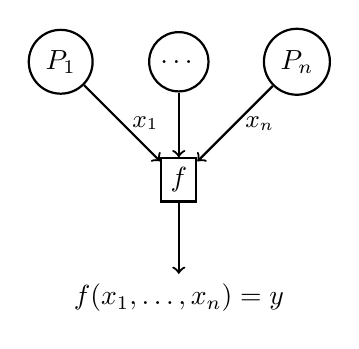
\begin{tikzpicture}[->,auto,node distance=1.5cm,
      thick,input node/.style={circle,draw},
      func node/.style={rectangle,draw}]

      \uncover<1,2,4>{%
      \node[input node] (1) {$P_1$};
      \node[input node] (2) [right of=1] {\ldots};
      \node[input node] (3) [right of=2] {$P_n$};
      }

      \uncover<3,4>{%
      \node[func node] (4) [below of=2] {$f$};

      \node (5) [below of=4] {$f(x_1, \ldots, x_n) = y$};
      }

      \uncover<4>{%
      \path[every node/.style={font=\small}]
      (1) edge node [right] {$x_1$} (4)
      (2) edge node {} (4)
      (3) edge node [right] {$x_n$} (4)
      (4) edge node {} (5);
      }
    \end{tikzpicture}
  \end{figure}
\end{frame}

\begin{frame}
  \begin{definition}[\Acl{MPC}, \acs{MPC}]
    \begin{itemize}
      \item \(n\) participants \(P_1, \ldots, P_n\).
      \item \(n\) secret inputs \(x_1, \ldots, x_n\).

        \pause{}

      \item A protocol \(\pi\) is executed by the participants.
      \item At the end of the protocol each participant learns \(y = f(x_1, 
          \ldots, x_n)\).

        \pause{}

      \item The participants executing \(\pi\) should be \emph{equivalent} to 
        giving \(x_1, \ldots, x_n\) to a trusted party \(T\) who computes 
        \(f(x_1, \ldots, x_n) = y\) and returns \(y\) to each participant.
    \end{itemize}
  \end{definition}

  \pause{}

  \begin{block}{Note}
    Each participant \(P_i\) learns no more about \(x_j\) (\(i\neq j\))
    than what is revealed by \(y\).
  \end{block}
\end{frame}

\begin{frame}
  \begin{itemize}
    \item In general this problem is solved.
    \item We can construct protocols for arbitrary functions \(f\).

      \pause{}

    \item Efficiency varies though.
    \item However, there are practically feasible protocols.

      \pause{}

    \item Sometimes we can use homomorphisms.
    \item But we can construct rather complex functions too.
  \end{itemize}
\end{frame}

\begin{frame}
  \begin{example}[Sugar beet auctions\footfullcite{MPCgoesLive}]
    \begin{itemize}
      \item Several thousand farmers produce sugar beets.
      \item These are sold to the monopoly Danisco, the sugar producer.

        \pause{}

      \item Contracts are allocated via a nation-wide exchange, a double 
        auction.

      \item A double auction contains multiple sellers and multiple buyers.

      \item The purpose is to find the \emph{market clearing price}.

    \end{itemize}
  \end{example}
\end{frame}

\begin{frame}
  \begin{example}[Sugar beet auctions, continued]
    \begin{itemize}
      \item Each buyer places a bid specifying how much he is willing to buy 
        \emph{at each potential price}.

      \item Each seller says how much they are willing to sell at each given 
        price.

        \pause{}

      \item The auctioneer computes the total supply and demand for each price.

      \item We want to find where supply equals demand.

        \pause{}

      \item When done, anyone who specified non-zero for this price may trade 
        at this price.
    \end{itemize}
  \end{example}
\end{frame}

\subsection{Zero-Knowledge Proofs of Knowledge}

\begin{frame}
  \begin{example}
    \begin{itemize}
      \item Alice must prove her identity to Eve.

      \item Eve has Alice's public key, and knows it belongs to Alice.

        \pause{}
        
      \item Alice wants to prove she is the owner of the private key belonging 
        to the public key that Eve has.

        \pause{}

      \item Eve asks Alice to sign the message \(m\), if the signature verifies
        under the public key Eve believes Alice.
        
    \end{itemize}
  \end{example}

  \pause{}

  \begin{alertblock}{Gaaahh!}
    \begin{itemize}
      \item Now Eve can show this message (chosen by Eve) with Alice's 
        signature on it!
      \item What if Eve's chosen message was \enquote{I give all my money to 
          Eve}?
    \end{itemize}
  \end{alertblock}
\end{frame}

\begin{frame}
  \begin{block}{The idea}
    \begin{itemize}
      \item Alice wants to prove that she knows the discrete logarithm \(x\) of 
        a value \(g^x\).

      \item She will do this without revealing \(x\) to Eve.
    \end{itemize}
  \end{block}
\end{frame}

\begin{frame}
  \begin{definition}[Schnorr's protocol\footfullcite{Schnorr}]
    \begin{itemize}
      \item Prover wants to prove knowledge of \(x\) for \(g^x = y\).

        \pause{}

      \item Prover commits to randomness \(r\), by sending \(t = g^r\).

        \pause{}

      \item Verifier replies with randomly chosen challenge \(c\).

        \pause{}

      \item After receiving \(c\), prover replies with \(s = r + cx\).

        \pause{}

      \item Verifier accepts if \(g^s = g^{r + cx} = g^r (g^x)^c = t y^c\).
    \end{itemize}
  \end{definition}
\end{frame}

\begin{frame}
  \begin{proof}[Proof outline]
    \begin{itemize}
      \item We need to prove \emph{completeness}: for all (most) statements the 
        verifier will accept.

        \pause{}

      \item We need to prove \emph{soundness}: for all (most) false statements 
        the verifier will reject.

        \pause{}

      \item We need to prove that it is zero-knowledge.
    \end{itemize}
  \end{proof}
\end{frame}

\begin{frame}
  \begin{block}{Zero-knowledge}
    \begin{itemize}
      \item Transcript for protocol: \((t, c, s)\).

      \item Probability for transcript occurring: \(\frac{1}{|R|}\cdot 
          \frac{1}{\deg g}\).

        \pause{}

      \item Simulate protocol: randomly choose \(c\), randomly choose \(s\), 
        compute \(t\) by \(g^s y^c\).

        \pause{}

      \item We see that we get the same probability distribution.
      \item Thus the simulated transcripts are indistinguishable from the real 
        ones.
    \end{itemize}
  \end{block}
\end{frame}


%%%%%%%%%%%%%%%%%%%%%%

\begin{frame}[allowframebreaks]
  \printbibliography{}
\end{frame}

